\documentclass{standalone}
\usepackage{tikz}
\begin{document}
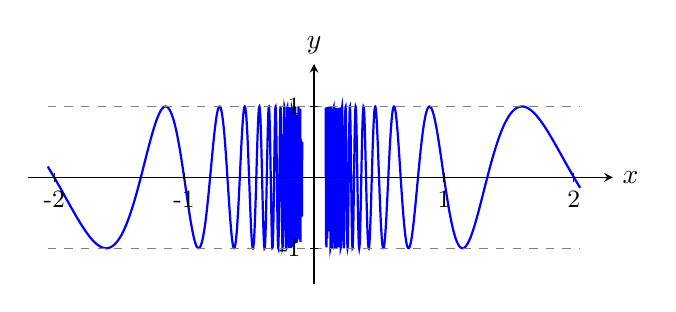
\begin{tikzpicture}[>=stealth, scale=0.75, x=2.2cm, y=1.2cm]
  % f(x) = sin(2*pi/x): oscillates between -1 and 1 near x = 0
  \begin{scope}
    \clip (-2.1,-1.3) rectangle (2.1,1.3);
    \draw[blue, thick, samples=900, smooth, domain=0.09:2.05]
      plot (\x, {sin(720/\x)});
    \draw[blue, thick, samples=900, smooth, domain=-2.05:-0.09]
      plot (\x, {sin(720/\x)});
  \end{scope}
  % Envelope guides
  \draw[dashed, gray] (-2.05,1) -- (2.05,1);
  \draw[dashed, gray] (-2.05,-1) -- (2.05,-1);
  % Axes
  \draw[->] (-2.2,0) -- (2.3,0) node[right] {$x$};
  \draw[->] (0,-1.5) -- (0,1.6) node[above] {$y$};
  % x-axis ticks
  \foreach \x in {-2,-1,1,2} {
    \draw (\x,0.06) -- (\x,-0.06) node[below, font=\small] {\x};
  }
  % y-axis ticks
  \foreach \y in {-1,1} {
    \draw (0.03,\y) -- (-0.03,\y) node[left, font=\small] {\y};
  }
\end{tikzpicture}
\end{document}
